%%%%%%%%%%%%%%%%%%%%%%%%%%%%%%%%%%%%%%%%%
% University Assignment Title Page
% LaTeX Template
% Version 1.0 (27/12/12)
%
% This template has been downloaded from:
% http://www.LaTeXTemplates.com
%
% Original author:
% WikiBooks (http://en.wikibooks.org/wiki/LaTeX/Title_Creation)
%
% License:
% CC BY-NC-SA 3.0 (http://creativecommons.org/licenses/by-nc-sa/3.0/)
%
% Instructions for using this template:
% This title page is capable of being compiled as is. This is not useful for
% including it in another document. To do this, you have two options:
%
% 1) Copy/paste everything between \begin{document} and \end{document}
% starting at \begin{titlepage} and paste this into another LaTeX file where you
% want your title page.
% OR
% 2) Remove everything outside the \begin{titlepage} and \end{titlepage} and
% move this file to the same directory as the LaTeX file you wish to add it to.
% Then add \input{./title_page_1.tex} to your LaTeX file where you want your
% title page.
%
%%%%%%%%%%%%%%%%%%%%%%%%%%%%%%%%%%%%%%%%%
%\title{Title page with logo}
%----------------------------------------------------------------------------------------
%	PACKAGES AND OTHER DOCUMENT CONFIGURATIONS
%----------------------------------------------------------------------------------------

\documentclass[12pt]{article}
\usepackage[toc,page]{appendix}
\usepackage[spanish]{babel}
\usepackage[utf8x]{inputenc}
\usepackage{amsmath}
\usepackage{graphicx}
\usepackage{fancyhdr}
\usepackage[colorinlistoftodos]{todonotes}
\usepackage{changepage}
\usepackage[font=scriptsize]{caption}
\usepackage[a4paper,bindingoffset=0.2in,left=1in,right=1in,top=1in,bottom=0.5in,footskip=.25in]{geometry}
\usepackage{cleveref}
\usepackage[hidelinks]{hyperref}
\usepackage{eurosym}
\usepackage{MathUnicode}
\usepackage{amssymb}
\usepackage{amsthm}
\usepackage{pdfsync}
\usepackage{color,xspace,hyperref}
\usepackage{changepage}
\usepackage{float}
\usepackage{caption}



\setlength{\arrayrulewidth}{1mm}
\setlength{\tabcolsep}{18pt}
\renewcommand{\arraystretch}{1.5}


\renewcommand{\labelitemii}{$\circ$}
\pagestyle{fancy}
\lhead{\textbf{Teoría del caos y fractales}}
\chead{\leftmark}
%\rhead{\includegraphics[width=2.8cm]{img/logo_memo}}
\rhead{\textbf{CyC}}

\newtheorem{theorem}{Teorema}
\newtheorem{lemma}{Lema}
\newtheorem{proposition}{Proposición}
\theoremstyle{definition}
\newtheorem{definition}{Definición}
\newtheorem{example}{Ejemplo}

\renewcommand{\headrulewidth}{0.5pt}

\begin{document}

\begin{titlepage}

\newcommand{\HRule}{\rule{\linewidth}{0.5mm}} % Defines a new command for the horizontal lines, change thickness here

\center % Center everything on the page

%----------------------------------------------------------------------------------------
%	HEADING SECTIONS
%----------------------------------------------------------------------------------------

\textsc{\LARGE Universidad Autónoma de Madrid}\\[1.5cm] % Name of your university/college
\textsc{\Large Complejidad y Computación}\\[0.5cm] % Major heading such as course name


%----------------------------------------------------------------------------------------
%	TITLE SECTION
%----------------------------------------------------------------------------------------

\HRule \\[0.4cm]
{ \huge \bfseries Teoría del Caos y fractales}\\[0.4cm] % Title of your document
\HRule \\[1cm]


%----------------------------------------------------------------------------------------
%	AUTHOR SECTION
%----------------------------------------------------------------------------------------


% If you don't want a supervisor, uncomment the two lines below and remove the section above
\Large \emph{Autoress:}\\
Alejandro \textsc{Villegas}\\ % Your name
Elena \textsc{Gutiérrez}\\ % Your name
Miguel Ángle \textsc{González-gallego} \\
Pedro \textsc{Valero}\\[1cm] % Your name

%----------------------------------------------------------------------------------------
%	LOGO SECTION
%----------------------------------------------------------------------------------------

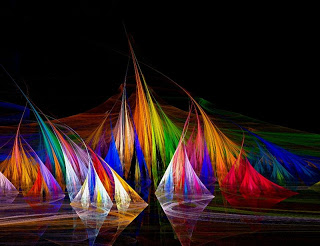
\includegraphics{img/Logo.jpg}\\ % Include a department/university logo - this will require the graphicx package

%----------------------------------------------------------------------------------------
%	DATE SECTION
%----------------------------------------------------------------------------------------

{\large \today}\\[1cm] % Date, change the \today to a set date if you want to be precise


%----------------------------------------------------------------------------------------

\vfill % Fill the rest of the page with whitespace

\end{titlepage}

\tableofcontents
\newpage

\section{Introducción}
Antes de comenzar a indagar en los fundamentos de la Teoría del Caos o en los fractales, debemos aclarar una serie de conceptos que aparecerán a lo largo de estos apuntes.

\begin{definition}[Teoría del Caos]
La teoría del Caos es la rama de las Matemáticas que estudia el comportamiento de sistemas dinámicos \textbf{deterministas} muy sensibles a los datos iniciales.
\end{definition}

Es importante destacar el hecho de que los sistemas han de ser deterministas pues, de lo contrario, estaríamos hablando de procesos aleatorios o impredecibles. La \textbf{idea clave} del concepto del Caos es que comprendemos el fenómeno y sabemos modelizarlo ``a la perfección'' pero el resultado futuro varía enormemente a partir de un pequeño cambio en los valores tomados del mundo real.

\begin{example}
A modo de ejemplo podemos suponer un fenomeno que venga modelizado por la ecuación:
\[z_{n+1} = f(z_n) \text{ siendo } f(x) = x^2+1\]

Para un $n=11$, que no parece ser algo demasiado grande, siendo $z$ un número complejo, supongamos que cometemos un error muy pequeño, de la forma: $ε=10^{-5}+10^{-5}i$ al medir $z_0$.

En estas condiciones, la diferencia entre el valor obtenido y el original es
\[f^{11}(ε)=1.4 \cdot 10^{181} + 1.13\cdot 10^{174}\]

Este ejemplo será estudiado con más detalle al hablar de los conjuntos de Mandelbrot
\end{example}

También es fundamental aclarar, aunque algunos lectores pueden tener ya una idea intuitiva, qué es un fractal.

\begin{definition}[Fractal]
Un fractal es un objeto geométrico cuya estructura básica, fragmentada o irregular, se repite a diferentes escalas.
\end{definition}

\section{Sistemas discretos}
Tiempo estimado de esta parte: 50 min\\
Referencia
\begin{itemize}
\item The Beauty of fractals temas 1,2,3,4 y 8.
\end{itemize}

\begin{definition}[Sistema dinámico]\label{def:sistemaDinamico}
Un sistema dinámico es un sistema cuyo estado evoluciona con el tiempo. Los sistemas físicos en situación no estacionaria son ejemplos de sistemas dinámicos, pero también existen modelos económicos, matemáticos y de otros tipos que son sistemas abstractos que son sistemas dinámicos.

Según las variables que intervienen en el sistema sean \textbf{discretas} (sólo tomen una serie de valores posibles) o \textbf{continuas} (pueden tomar cualquier valor dentro de un intervalo), así lo será el sistema.
\end{definition}

Un sistema dinámico se define como \textbf{determinista} si existe una ecuación que nos permite conocer \textbf{teóricamente} la evolución del sistema con total precisión.


\subsection{Ecuaciones en diferencias.}
% Pedro: Esta no es mi parte pero he escrito esto y al final me he dado cuenta de que se corresponde con sistemas discretos, no continuos. Así que lo pongo por aquí.

\begin{definition}[Ecuación en diferencias]
Una ecuación en diferencias es una expresión del tipo:
\[G(n,f(n),f(n+1),...,f(n+k))=0, \ \forall n \in \mathbb{Z}\]
donde $f$ es una función definida en $\mathbb{Z}$.
\end{definition}

\begin{example}
La ecuación en diferencias de primer orden:
\[X_{t+1} = F(X_t)\]
constituye un ejemplo de sistema dinámico determinista, siendo $F(x)$ una función conocida.
\end{example}


% Todo lo que viene a continuación viene de http://ltcconline.net/greenl/courses/204/firstOrder/differenceEquations.htm

A simple vista puede parecer que el ejemplo mencionado no es una ecuación en diferencias, puesto que no se aprecia ninguna derivada en la ecuación. No obstante, podemos escribir:
\[X'(t)=g(X(t)) \implies \lim_{h\to 0} \frac{X(t+h)-X(t)}{h}\]

Puesto que los valores posibles de $t$ y $h$ son enteros, lo más pequeño que puede ser $h$ sin llegar a ser $0$ es $h=1$ con lo que tenemos:
\[g(X(t))=X'(t)=X(t+h)-X(t)=ΔX(t) \implies X(t+h) = X(t) +ΔX(t) \implies \atop F(X(t)) = X(t) + ΔX(t)\]

Por tanto, encontrar la función $X(t)$ que resuelve el sistema planteado en el ejemplo es equivalente a resolver la ecuación:
\[X(t+1)=X(t)+ΔX(t)\]
que, claramente, es una ecuación en diferencias.

\subsection{Procesos de Verhulst. Period doubling, bifurcaciones.}
\subsection{Ecuación logística}
\subsection{$x=x^2+c$. Julia sets. Mandelbrot set.}
\subsection{Fractales/dimensión de Hausdorlf/dimensión fractal}
\subsection{Polvo de Cantor} No aparece en The Beauty of fractals (en algún otro libro de la bibliografía está).
\subsection{Ecuaciones de Volterra}

%%%%%%%%%%%%%%%%%%%%%%%%%%%%%%%%%%%%%%%%%%%%%%%%%%%%%%%%%%
%%%%%%%%%%%%%%%%%%%%%%%%%%%%%%%%%%%%%%%%%%%%%%%%%%%%%%%%%%
%%%%%%%%%%%%%%%%%%%%%%%%%%%%%%%%%%%%%%%%%%%%%%%%%%%%%%%%%%
%%%%%%%%%%%%%%%%%%%%%%%%%%%%%%%%%%%%%%%%%%%%%%%%%%%%%%%%%%
%%%%%%%%%%%%%%%%%%%%%%%%%%%%%%%%%%%%%%%%%%%%%%%%%%%%%%%%%%
%%%%%%%%%%%%%%%%%%%%%%%%%%%%%%%%%%%%%%%%%%%%%%%%%%%%%%%%%%
%%%%%%%%%%%%%%%%%%%%%%%%%%%%%%%%%%%%%%%%%%%%%%%%%%%%%%%%%%
%%%%%%%%%%%%%%%%%%%%%%%%%%%%%%%%%%%%%%%%%%%%%%%%%%%%%%%%%%
%%%%%%%%%%%%%%%%%%%%%%%%%%%%%%%%%%%%%%%%%%%%%%%%%%%%%%%%%%

\section{Sistemas continuos}
% Tiempo estimado de esta parte: 70 min.\\
% Referencia
% \begin{itemize}
% \item CHAOS: An introduction to dynamical systems temas 7,8,9 y 11.
% \item Elegant Chaos
% \end{itemize}

\subsection{Sistemas dinámicos deterministas, ecuaciones diferenciales}

Los sistemas dinámicos continuos deterministas \ref{def:sistemaDinamico} vienen modelizados por ecuaciones diferenciales.

En lugar de expresar el estado actual en función de un estado anterior, las ecuaciones diferenciales tratan de expresar la \emph{tasa de cambio} del estado actual en función del estado actual. La tasa de cambio de una cierta función es su \emph{derivada}. Tenemos la siguiente definicón general de ecuación diferencial.

\begin{definition}
Una ecuación diferencial es una fórmula matemática que relaciona una función con sus derivadas.
\end{definition}

\begin{example}\label{ex:calor}
Un ejemplo de este tipo de dependencia es la \emph{Ley del calor de Newton}. Si consideramos $x$ como la diferencia de temperatura entre el objecto caliente y la temperatura ambiente del aire que lo rodea, la tasa de cambio de esta diferencia de temperatura es inversamente proporcional a la diferencia de temperatura. En términos de ecuaciones diferenciales, diremos:
\begin{equation}
x' = ax~~~con~~ a<0
\end{equation}

La solución de esta ecuación viene dada por:
\begin{equation}
x(t) = c x(0)e^{at}
\end{equation}

Esto quiere decir que, la diferencia de temperatura $x$ decrece exponencialmente con el tiempo $t$. Se trata de una ecuación  de \emph{primer orden}, puesto que el \emph{orden} de la derivada más alto que aparece es el de la \emph{primera} derivada, y \emph{lineal} porque la relación entre las funciones $x'$ y $x$ en la ecuación es \emph{lineal}.
\end{example}

En el siguiente ejemplo, veremos un caso de ecuación diferencial \emph{de segundo orden} \emph{no lineal}.

\begin{example}
En este caso estudiaremos el movimiento de un péndulo \emph{bob}, el movimiento de un péndulo que tiene en su extrem un peso y que cuelga de un soporte que limita su movimiento a lo largo de un círculo. La aceleración que experimenta este péndulo es tangente a la dirección dle movimiento y proporcional a la componente de la fuerza gravitatoria sobre la dirección tangencial. Si representamos con $x$ la posición angular (eso es la razón entre la longitud del arco que forma el péndulo con la vertical y la longitud del péndulo), entonces la relación entre su derivada segunda y ésta viene dada por:
\begin{equation}
x'' = -sinx
\end{equation}

Esta ecuación es una de las más importantes en ciencia y se trata de una ecuación de \emph{segundo orden}, puesto que el \emph{orden} de la derivada más alto que aparece es el de la \emph{segunda} derivada, y \emph \emph{no lineal}, porque la relación entre las funciones $x''$ y $x$ en la ecuación es \emph{no lineal}.
\end{example}


En ambos ejemplos, buscamos soluciones de la forma $x(t)$ donde $t$ denota el tiempo y $x(t)$, por tanto, una cierta magnitud física que varía en función del tiempo: en el primer ejemplo, la diferencia de temperatura; en el segundo ejemplo, la posición angular. Es por eso que, consideramos que $x$ es una variable \emph{dependiente}. Si la variable \emph{independiente} $t$ no aparece explicítamente en la ecuación, como es el caso en los dos ejemplos anteriores, hablaremos de ecuaciones diferenciales \emph{autónomas}. Si $t$ aparece explícitamente en la ecuación como es el caso de la ecuación del \emph{péndulo amortiguado} (el columpio):
\begin{equation}
x'' = -cx'-sinx+\rho~sint
\end{equation}
entonces hablaremos de ecuaciones diferenciales \emph{no autónomas}.

Recapitulando las nociones vistas hasta ahora tendríamos la siguiente clasificación de las ecuaciones diferenciales:

\begin{itemize}
\item Según el orden de las derivadas que aparezcan en la expresión:
	\begin{itemize}
	\item Primer orden
	\item Segundo orden
	\item ...
	\end{itemize}
\item Según la relación entre la función $x$ y sus derivadas
	\begin{itemize}
	\item Lineales
	\item No lineales
	\end{itemize}
\item Según si aparece explicítamente la variable $t$ en la ecuación
	\begin{itemize}
	\item Autónomas
	\item No autónomas
	\end{itemize}
\end{itemize}

Si recuperamos el ejemplo \ref{ex:calor}, teníamos que las soluciones eran de la forma:
\begin{equation}
x(t) = c x(0)e^{at}
\end{equation}
 La $c$ es una constante en $\mathbb{R}$. Esto quiere decir que, la ecuación diferencial planteada en \ref{ex:calor} tiene \emph{infinitas} soluciones, a menos que especifiquemos un \emph{valor inicial} de la $x$. Al hacer esto estaremos \emph{seleccionando} una de las soluciones dentro de la familia de soluciones (GRAFICA FAMILIA DE SOLUCIONES p.276). En nuestro caso, podemos establecer:

\begin{equation}
x(0) = x_0
\end{equation}

y por tanto, la solución particular de nuestro problema sería:

\begin{equation}
x(t) = x_0e^{at}.
\end{equation}

En general, a los problemas experesados en forma de ecuación diferencial más dato inicial, los denominaremos \emph{problemas de valor inicial}.

A seguir con:

\begin{itemize}
\item Hablar de ls GRAFICA FAMILIA DE SOLUCIONES DE E. NO LINEALES (p.279)
\item Concepto de solución de equilibrio
\item Concepto de trayectorias/puntos atractores
\item Concepto de trayectorias/puntos ?repelentes?
\item Concepto de existencia, unicidad y dependencia continua (que no es lo mismo que dependencia ?sensitiva?)
\item Ejemplos de ecuaciones de dimension>1 y sus soluciones.
\item Sistemas no lineales y pérdida de la posibilidad de resolver explicitamente (hay más pegas, ver cuáles).
\end{itemize}
\textcolor{red}{No se si poner este ejemplo es demasiado. Creo que si queremos hablar de ecuaciones diferenciales debemos explicar qué son y cómo se usan. No veo mal si decidimos quitarlo por completo. Es un copy and paste xd}

\begin{example}[Curva de persecución]
Supongamos que una liebre que se encuentra inicialmente en el origen de coordenadas comienza a huir, con velocidad $V_L$ y en el sentido positivo del eje de ordenadas, de un perro que inicialmente tiene la posición $(0,D)$ y que comienza a perseguirle con velocidad $V_P$.

\begin{figure}[hbtp]
\centering
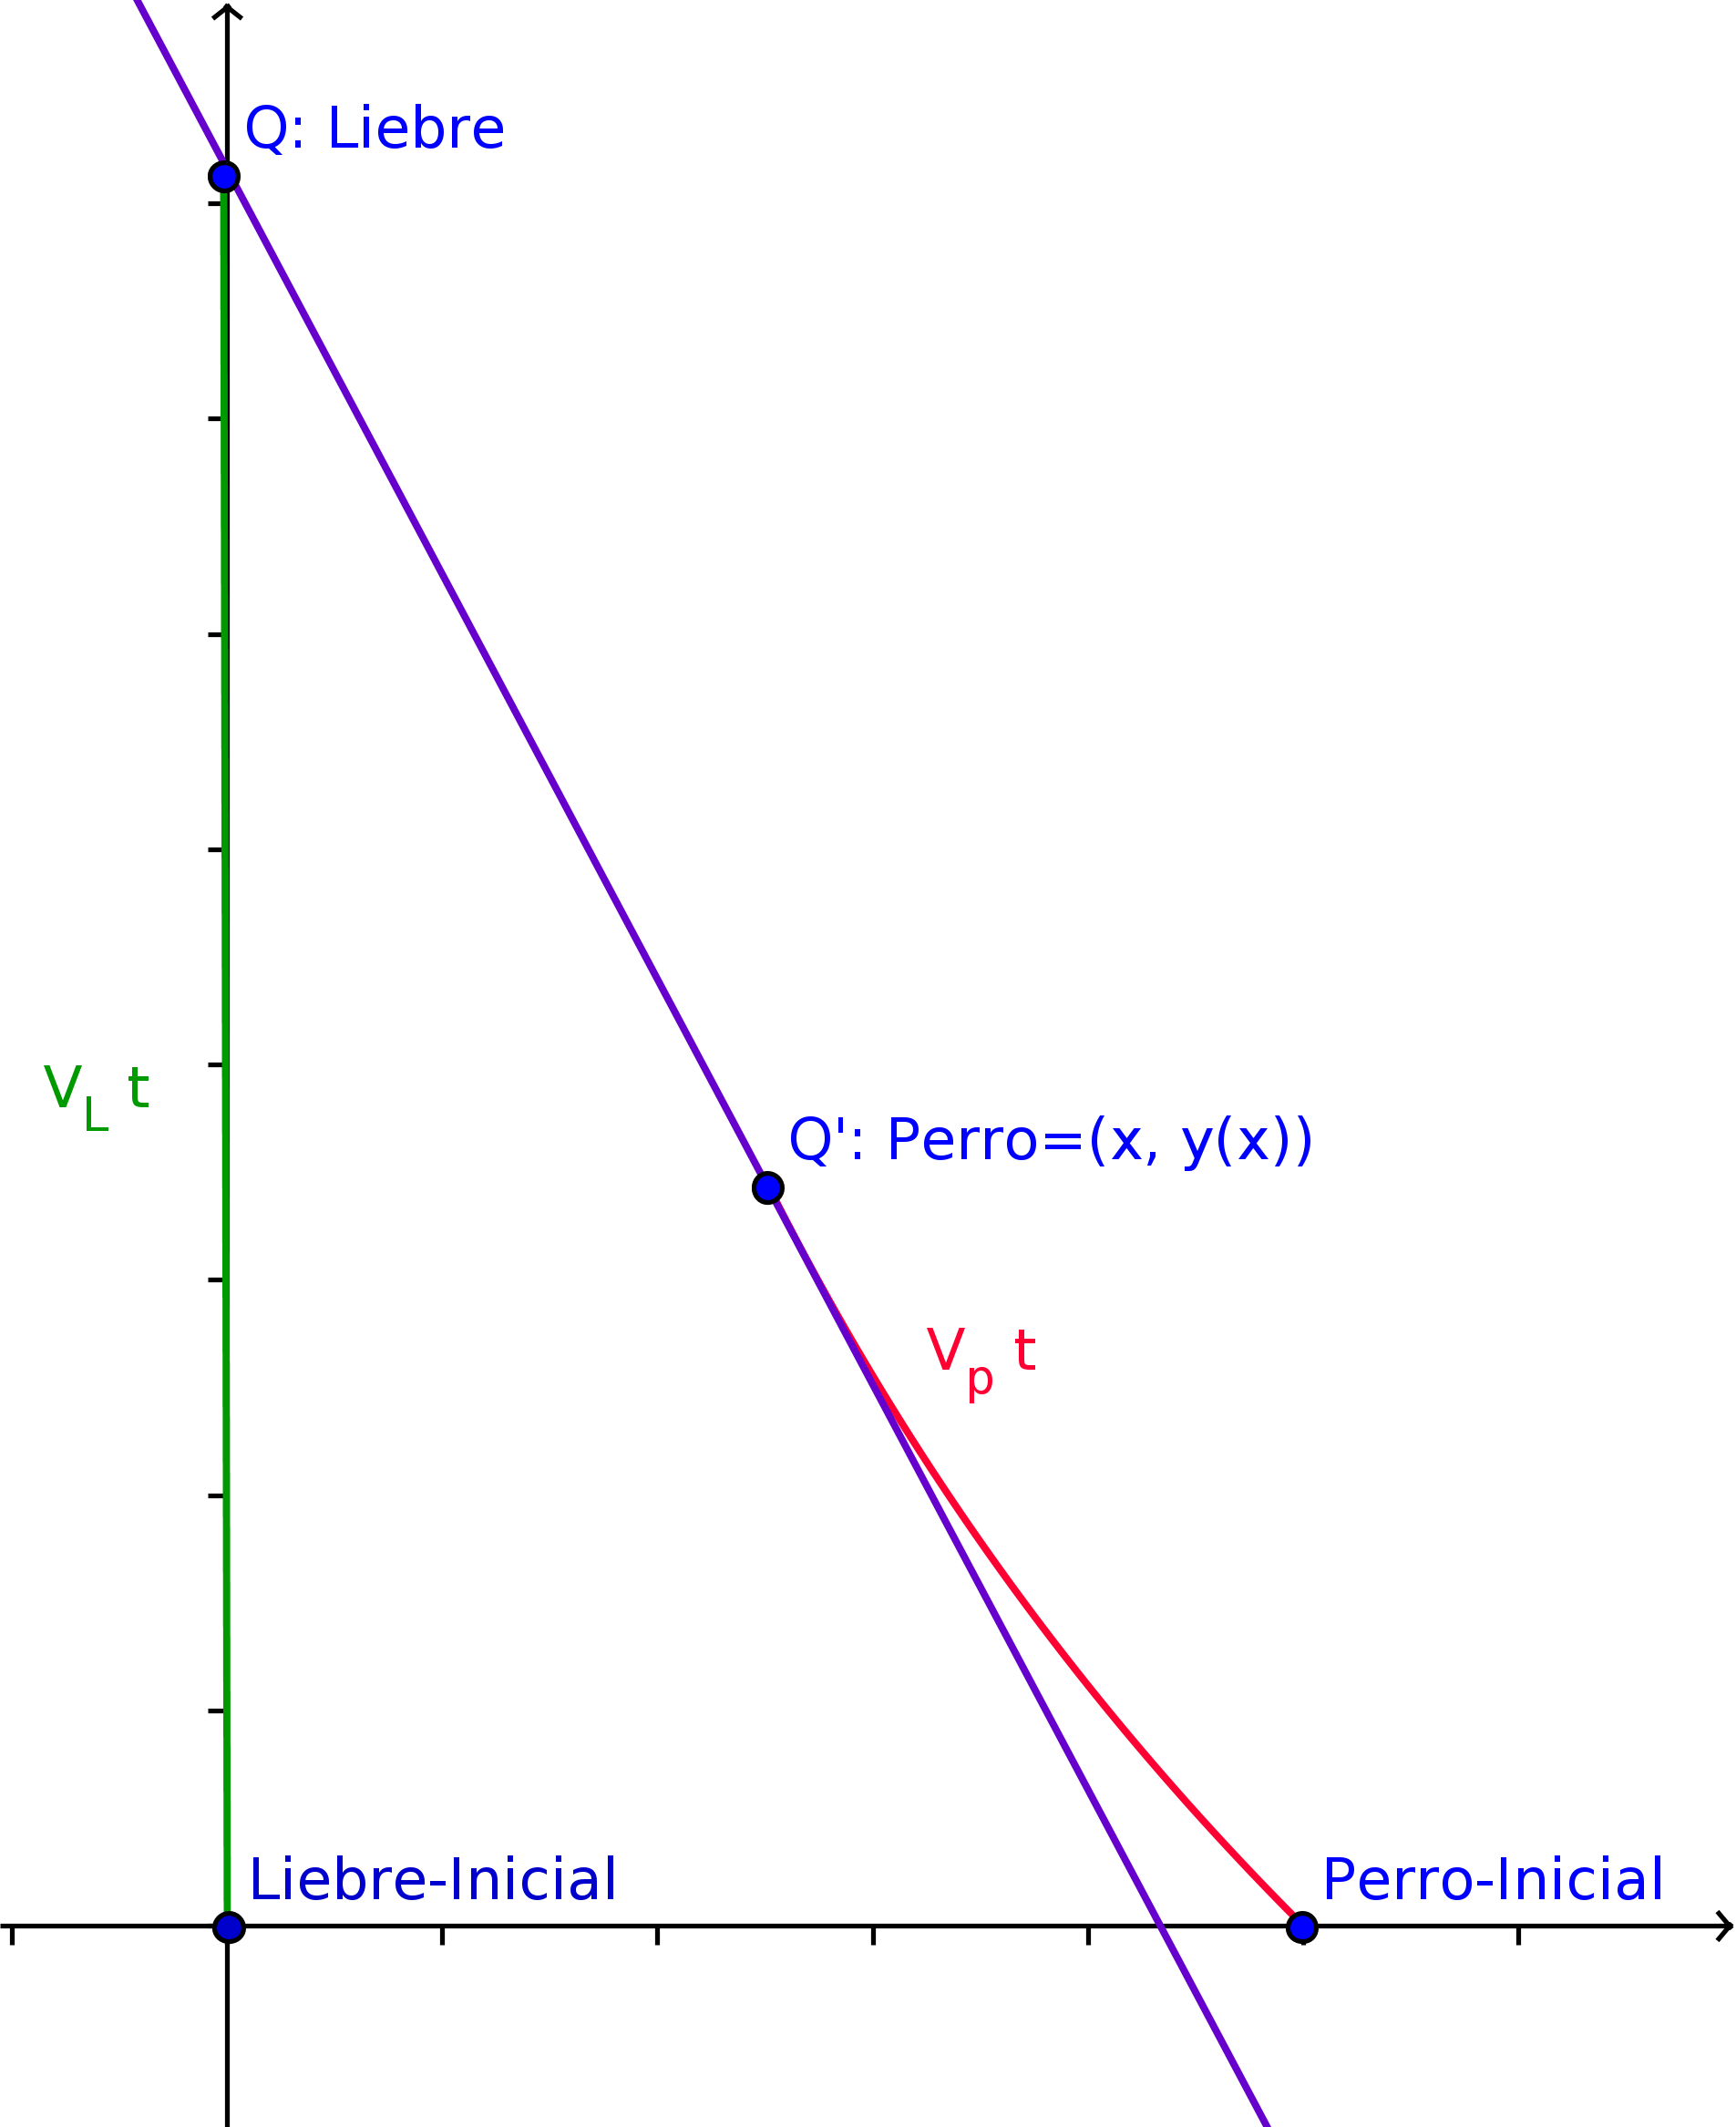
\includegraphics[width = 0.4\textwidth]{img/perro-liebre.png}
\end{figure}

Llamaremos $Q$ a la posición de la liebre en cada instante y $Q^\prime:(x,y(x))$ a la posición del perro.

Observamos que el perro, al perseguir a la liebre, siempre lo hace mirándole, por tanto, en cada instante, la recta tangente a la curva que describe el perro al perseguir a la liebre pasa por $Q$ y por $Q^\prime$.

Como dato adicional tenemos que la distancia recorrida por la liebre es $V_Lt$ y la distancia recorrida por el perro es $V_Pt$, por tanto, en cada instante, la liebre está en la posición $(0, V_Lt)$.

Tenemos pues:

\begin{itemize}
\item Vector tangente: $(1, y^\prime(x))$
\item Recta tangente: $(x,y) + \lambda(1, y^\prime(x))$
\item Como sabemos que la recta tangente pasa por $Q$ cuando $\lambda = -x$ (porque $Q$ está en el eje de ordenadas y ha de tener la primera coordenada igual a cero) tenemos que \\$Q=(0, y-xy^\prime(x))$ y además que $Q=(0, V_Lt)$ por tanto $V_Lt = xy^\prime(x)$
\item La distancia recorrida por el perro es $V_Pt =\int_x^D{\sqrt{1+(y^\prime(s))^2ds}}$
\item Despejando $t$ de ambas ecuaciones e igualando términos tenemos que $\frac{V_P}{V_L}(y-xy^\prime(x))=\int_x^D{\sqrt{1+(y^\prime(s))^2ds}}$
\item Derivando ambos términos y utilizando el cambio $p=y^\prime$ llegamos a $\frac{V_p}{V_L}xp^\prime=\sqrt{1+p^2}$
\item Integrando: $\sqrt{1+p^2}+p = e^{C_1}x^\frac{V_L}{V_T}$
\item Despejando de esta ecuación obtenemos $p$ y por tanto $y^\prime$, habrá que calcular la constante de integración y volver a integrar y a calcular la nueva constante de integración para obtener $y$, por lo que necesitaremos dos datos adicionales para efectuar este cálculo:$$y(D)=0$$ $$y^\prime(D)=0$$
\end{itemize}
La expresión que se obtiene depende de las velocidades $V_L$ y $V_P$. Vamos a simplificar el problema suponiendo $D=1$. Tenemos tres casos distintos:
\begin{itemize}
\item \textbf{Caso 1:} $V_L=V_P$\\
En este caso se tiene $y^\prime(x) = \frac{1}{2}(x-\frac{1}{x})$ de donde obtenemos $y(x) = \frac{1}{2}(\frac{x^2}{2}-ln(x))+C_2$ y utilizando el dato $y(1) = 0$ podemos hallar $C_2=\frac{-1}{4}$.\\Tenemos como solución $y(x) = \frac{x^2}{4}-\frac{1}{2}ln(x)-\frac{1}{4}$.\\ Una vez obtenida la expresión, podemos hallar la distancia entre la liebre y el perro, que dependerá de la posición del perro: $d=\sqrt{x^2+x^2(y^\prime(x))^2}$.\\ Como el perro va describiendo una curva y la liebre una recta vemos que el perro se va acercando poco a poco a la liebre. Sin embargo, cuando $x\longrightarrow 0^+$ vemos que la curva que describe el perro ``se parece'' cada vez más a una recta y por tanto en el infinito la distancia de separación se mantendrá constante.\\
Tenemos pues que $$\lim_{x\to 0^+} d = \frac{1}{2}$$
\item \textbf{Caso 2:} $V_L < V_P$\\
Tenemos la expresión $$y=\frac{1}{2}(\frac{x^{\frac{V_L}{V_P}+1}}{\frac{V_L}{V_P}+1}-\frac{x^{1-\frac{V_L}{V_P}}}{1-\frac{V_L}{V_P}})+C_3$$
En esta ocasión tenemos que el perro alcanza a la liebre. Sabiendo que $y(1) = 0$ podemos calcular la constante $C_3$ y el valor de $y(0)$ es el punto de captura.
\item \textbf{Caso 3} $V_L > V_P$\\
En este caso el perro no llega a alcanzar nunca a la liebre, que es más rápida. Al igual que hemos calculado la distancia de separación en el caso 1 y el punto de captura en el caso 2, en este caso lo interesante será calcular la tasa de separación entre la liebre y el perro.
\end{itemize}
\end{example}

\subsection{Espacio de estados/fases}

Un concepto muy útil a la hora de trabajar con ecuaciones diferenciales son los \textbf{diagramas de fases}.

Tomemos la ecuación diferencial
\[y(x)'=f(y(x))\]
donde la función $f$ viene dada por la siguiente gráfica

\begin{figure}[hbtp]
\centering
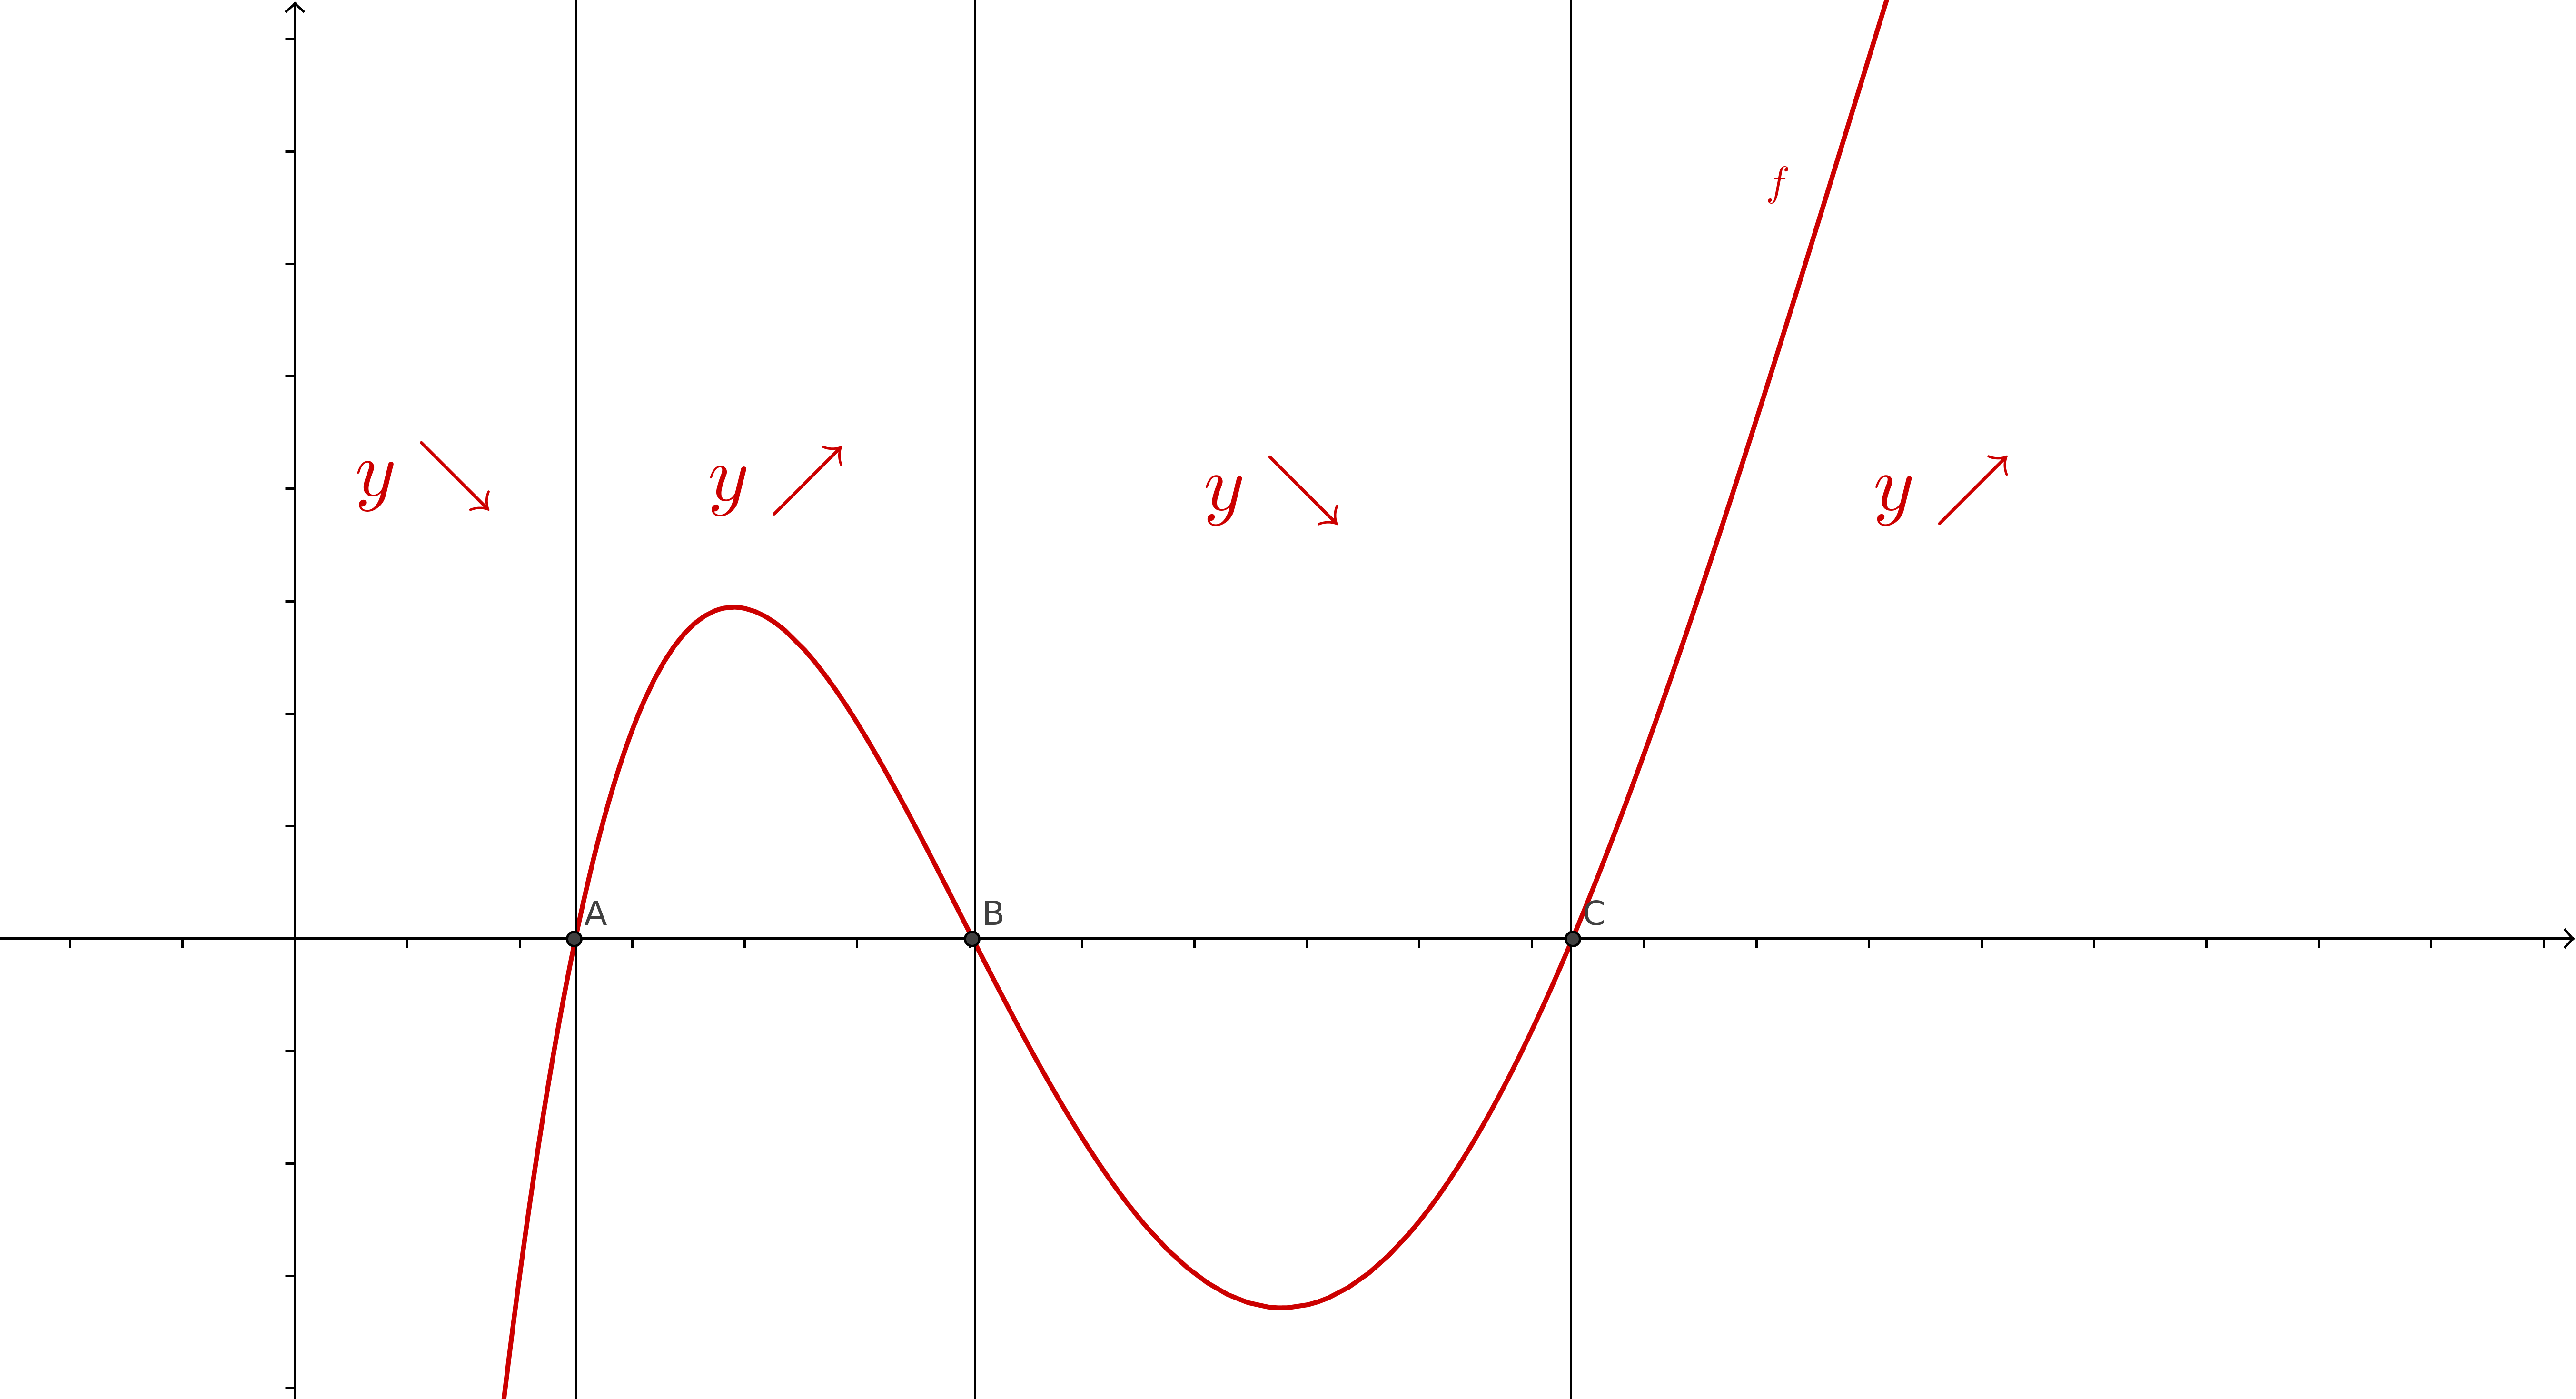
\includegraphics[width = 0.8\textwidth]{img/propiedades-autonomas.png}
\end{figure}

Podemos observar que si nos situamos ``a la izquierda de $a$'' o ``entre $b$ y $c$'' la función $y$ es decreciente. Del mismo modo, si nos situamos ``entre $a$ y $b$'' o ``a la derecha de $c$'' la función será creciente mientras que en los puntos $a, b$ y $c$ la función ni crece ni decrece. Esta información queda recogida en el siguiente diagrama de fases:

\begin{figure}[hbtp]
\centering
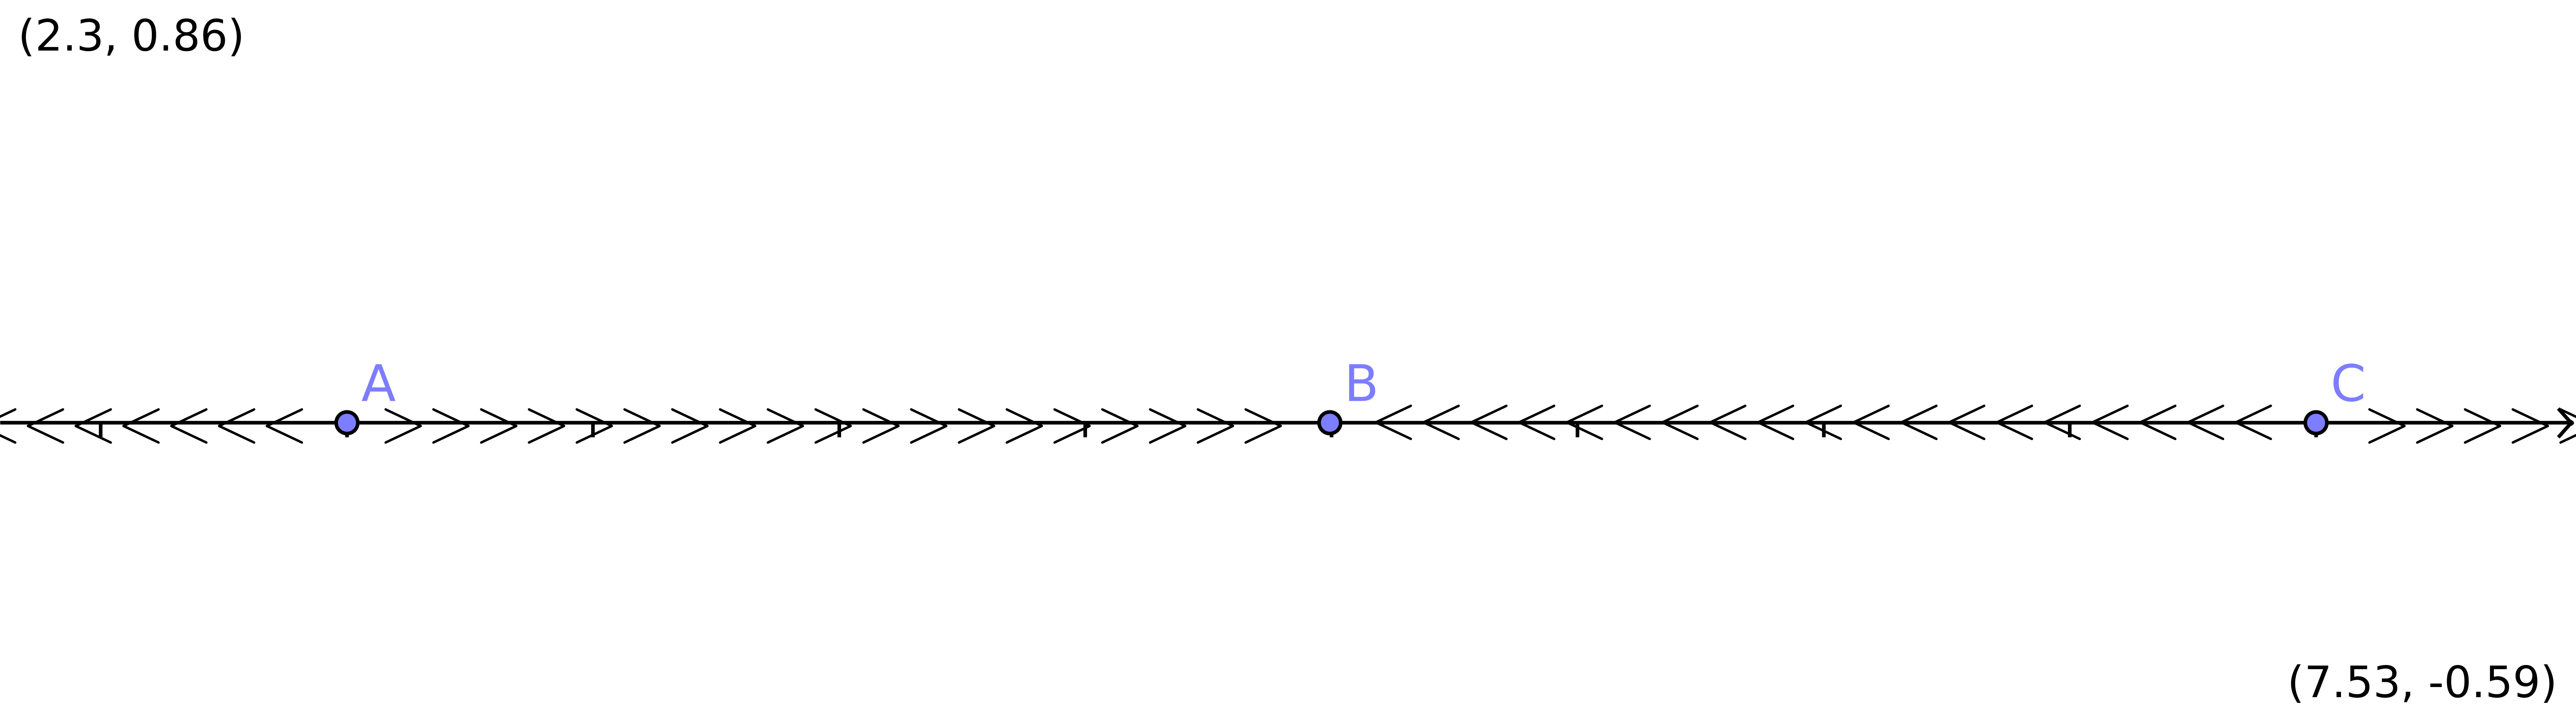
\includegraphics[width = 0.8\textwidth]{img/diagrama-fases.png}
\end{figure}

En este caso diremos que $a$ y $c$ son puntos \textbf{inestables} pues una pequeña perturbación hará que nos alejemos de ellos. Igualmente, diremos que $b$ es un punto \textbf{estable} porque una pequeña perturbación hará que volvamos de nuevo a desplazarnos hacia $b$.

\subsection{Oscilaciones}
\subsection{Sistemas disipativos: atractores}
\subsection{Flujos, compresibles o no}
\subsection{Atractores extraños: caos}
Hay que hablar de Atractores de Lorentz (artículo relacionado)
\subsection{Exponentes de lyapunov}
Hay que incluir algo.
\subsection{Ejemplos de sistemas}
Para los ejemplos: Non linear dynamic and chaos.
\subsection{Lorenz Volterra}
Ecuaciones en Non linear dynamic and chaos.

%%%%%%%%%%%%%%%%%%%%%%%%%%%%%%%%%%%%%%%%%%%%%%%%%%%%%%%%%%
%%%%%%%%%%%%%%%%%%%%%%%%%%%%%%%%%%%%%%%%%%%%%%%%%%%%%%%%%%
%%%%%%%%%%%%%%%%%%%%%%%%%%%%%%%%%%%%%%%%%%%%%%%%%%%%%%%%%%
%%%%%%%%%%%%%%%%%%%%%%%%%%%%%%%%%%%%%%%%%%%%%%%%%%%%%%%%%%
%%%%%%%%%%%%%%%%%%%%%%%%%%%%%%%%%%%%%%%%%%%%%%%%%%%%%%%%%%
%%%%%%%%%%%%%%%%%%%%%%%%%%%%%%%%%%%%%%%%%%%%%%%%%%%%%%%%%%
%%%%%%%%%%%%%%%%%%%%%%%%%%%%%%%%%%%%%%%%%%%%%%%%%%%%%%%%%%
%%%%%%%%%%%%%%%%%%%%%%%%%%%%%%%%%%%%%%%%%%%%%%%%%%%%%%%%%%
%%%%%%%%%%%%%%%%%%%%%%%%%%%%%%%%%%%%%%%%%%%%%%%%%%%%%%%%%%

\section{Aplicaciones}
Tiempo estimado de esta parte: 30 min.\\
Referencia
\begin{itemize}
\item Guide to Chaos
\end{itemize}
\subsection{Generación gráfica de conjuntos de Julia}
\subsection{Ejemplos gráficos de explorar el conjunto de Mandelbrot}
\subsection{Caos y criptografía}
\subsection{Compresión fractal}
\subsection{Antenas fractales}
\subsection{Aeronáutica y fluidos}

%%%%%%%%%%%%%%%%%%%%%%%%%%%%%
%%%%%%
%%%%%%
%%%%%%
%%%%%%%%%%%%%%%%%%%%%%%%%%%%%
\newpage

\begin{thebibliography}{1}
\bibitem{B1165 SPR}Dprott, J.C, Elegant Chaos
\bibitem{C4260 PEI}Peitgen, H-O, Richter, P.H., The Beauty of Fractals.
\bibitem{B1165 NEW}Hall, Nina, Guide to Chaos
\bibitem{B0240 STR}Strogatz, S.H. Nonlinear Dynamics and Chaos,
\bibitem{B1165 ALL}Alligood, K.T. et al, CHAOS: An introduction to dynamical systems
\end{thebibliography}

\end{document}